%
%  Erik Olsen
%
\documentclass[12pt,fullpage]{article}
\usepackage{fullpage}                                        % use all of the page for text 
\usepackage{psfrag}                                          % LaTeX graphics tool
\usepackage{pslatex}                                         % avoids the default cmr font
\usepackage{graphicx}                                        % graphics package 
\usepackage{epsfig}                                          % figures
\usepackage{epsfig} 
\usepackage{hyperref}
\usepackage{color}

\begin{document}

\noindent
{\bf Chi distribution} (from \color{blue}\url{http://www.math.wm.edu/~leemis/chart/UDR/UDR.html}\color{black})

\noindent
The shorthand $X \sim {\chi}(n)$ is used to indicate that the
random variable $X$ has the $\chi$ (chi) distribution with $n$ degrees of freedom, where $n$ is a positive integer.
A $\chi$ random variable $X$ with $n$ degrees of freedom has probability density function 
$$
f(x) = \frac{1}{2 ^ {n / 2 - 1}\Gamma(n / 2)} x ^ {\kern 0.04em n-1}e ^ {-x ^ {\kern 0.04em 2} / 2} \qquad \qquad x>0.
$$
The probability density function, where $n=1,\, 2,\, {\rm and}\  8$ is illustrated below.
{\begin{figure}[h!]
\begin{center}
\psfrag{lab1}{$n = 1$}
\psfrag{lab2}{$n = 2$}
\psfrag{lab3}{$n = 8$}
\psfrag{labx}{$x$}
\psfrag{labf}{$f(x)$}
\includegraphics[width=3.2in]{ChiPlot.ps}
\end{center}
\end{figure}}\\
The cumulative distribution function of $X$ can be written as an integral that can't be
evaluated in closed form.
The expected value of $X^k$ is
$$
E\left[ X ^ k \right] = \frac{2 ^ {k / 2} \Gamma(k / 2 + n / 2)}{\Gamma(n / 2)}
$$
for $k = 1, \, 2, \, \ldots \,$.
Using this result, the mean and variance are
$$
E[X] = \frac {\sqrt {2} \kern 0.08em\Gamma  \left( 1 / 2 + n / 2 \right) }{\Gamma  \left(n / 2 \right) } \qquad \qquad 
V[X] = n - \kern 0.04em \mu ^ 2 
$$
because
$$
E\left[ X ^ 2 \right] = \frac{2 \Gamma(n / 2 + 1)}{\Gamma(n / 2)} = n.
$$
The skewness and kurtosis are also written in terms of the gamma function.
%  $$ 
%  E\left[ \left( \frac{X - \mu}{\sigma} \right) ^ {\kern -0.08em 3} \right] =\frac{\mu}{\sigma ^ 3}\left(1 - 2 \kern 0.04em \sigma ^ 2\right)\qquad \qquad
%  E\left[ \left( \frac{X - \mu}{\sigma} \right) ^ {\kern -0.08em 4} \right] = \frac{2}{\sigma ^ 2}\left(1 - \mu\kern 0.04em\sigma\kern 0.04em\gamma_1 - \sigma ^ 2\right)
%  $$
The mode is $\sqrt{n-1}$.

\vspace{0.1in}

\noindent
{\bf APPL verification:}
The APPL statements
\begin{verbatim}
X := ChiRV(n);
Mean(X);
Variance(X);
Skewness(X);
Kurtosis(X);
\end{verbatim}
verify the population mean, variance, skewness, kurtosis, and moment generating function.
\end{document}
